Im Rahmen der vorliegenden Arbeit konnte die Funktionalität des Moduls \texttt{mpshift} deutlich erweitert und die Effizienz bei den Berechnungen maßgeblich gesteigert werden. In Abbildung \ref{abb:neue_programmstruktur} ist eine schematische Darstellung der Programmstruktur des Moduls \texttt{mpshift} mit den in dieser Arbeit vorgenommenen Erweiterungen und Modifikationen gezeigt. Durch die Implementierung des \acfp{cosmo} besteht nun die Möglichkeit, Umgebungseffekte bei der Berechnung von chemischen Abschirmungskonstanten einzubeziehen. Zusätzlich ermöglicht dieses Modell die Kompensation von Gegenionen, was insbesondere für hoch geladene anionische Verbindungen wichtig ist. Ohne eine solche Ladungskompensation kommt es oft bereits bei der Berechnung der Grundzustandswellenfunktion zu einem schlechten Konvergenzverhalten bzw. zu überhaupt keiner Konvergenz. Um konsistente Resultate zu erhalten, war es wichtig, diese Methode auch auf die Berechnung von chemischen Abschirmungskonstanten zu übertragen. Zusätzlich wurde das \acf{dcosmors} implementiert und in einer ausführlichen Studie mit dem \ac{cosmo} verglichen. Dafür wurden 61 $^{13}$C-chemische Verschiebungen organischer Moleküle in 12 unterschiedlichen Lösungsmitteln berechnet und mit experimentellen Daten verglichen. Neben diesen beiden Modellen wurden weitere Möglichkeiten zur Berücksichtigung von Lösungsmitteleffekten -- beispielsweise das explizite Berechnen von Lösungsmittelmolekülen -- anhand der Solvatationsverschiebung von Aceton beim Übergang von der Gasphase in eine wässrige Lösung untersucht. Insbesondere das \ac{dcosmors} erweist sich hierbei als besonders vorteilhaft und kann die experimentell gemessenen Verschiebungen gut reproduzieren. Im Allgemeinen kann bei den in dieser Arbeit untersuchten Beispielen jedoch kein klarer Favorit der beiden Methoden ausgemacht werden.

Die Implementierung von \acfp{ecp} ermöglicht nun die Berechnung von chemischen Abschirmungskonstanten in Molekülen, welche schwere Elemente beinhalten, ohne große All-Elektronen-Basissätze verwenden zu müssen. Auf diese Weise wird zusätzlich die Auswirkung relativistischer Effekte auf die Abschirmungskonstanten der Nachbaratome schwerer Elemente berücksichtigt. Die Eichinvarianz der Implementierung wurde anhand der chemischen Abschirmungskonstanten in Co(ppy)$_3$ (ppy=2-Phenylpyridin) demonstriert. Aufgrund der fehlenden Rumpfelektronen sind die berechneten chemischen Abschirmungskonstanten für die Atome mit \acp{ecp} etwa ein bis zwei Größenordnungen kleiner als die gemessenen Daten und damit prinzipiell unphysikalisch. Ihre relative Lage zueinander korreliert jedoch gut mit experimentell gemessenen chemischen Verschiebungen, solange ähnliche Systeme betrachtet werden.

Das Modul \texttt{mpshift} kann nun ebenfalls die Response der Wellenfunktion auf ein äußeres Magnetfeld, welche zur Berechnung von \ac{vcd}-Spektren benötigt wird, bereitstellen. Die eigentliche Berechnung der \ac{vcd}-Spektren wurde in das im Modul \texttt{aoforce} implementiert. Der Vergleich zwischen dem experimentellen \ac{vcd}-Spektrum und den simulierten \ac{vcd}-Spektren von \acl{cpa} zeigt, dass die effiziente Basissatz/Funktional-Kombination def2-SV(P)/BP86 qualitativ gleichwertige Spektren liefert wie die deutlich aufwändigere Kombination def2-TZVP/B3LYP. Die effiziente Implementierung aus der vorliegenden Arbeit erlaubt beispielsweise die Berechnung der \ac{vcd}-Spektren von großen $I$-symmetrischen Fullerenen. Darunter ist das C$_{620}^{2+}$ mit 8680 Basisfunktionen das bislang größte System, für welches ein \ac{vcd}-Spektrum berechnet wurde.

Des Weiteren wurde das Modul \texttt{mpshift} in Zusammenarbeit mit Fabian Mack im Rahmen seiner Masterarbeit um die Möglichkeit erweitert, chemische Abschirmungskonstanten mithilfe von \ac{mgga}-Funktionalen zu berechnen. 

\bigskip
Durch die Implementierung der \ac{ri}- und \ac{marij}-Verfahren konnte eine hoch effiziente Berechnung des Coulombbeitrages erreicht werden. Dies führt beispielsweise bei der Berechnung der chemischen Abschirmungskonstanten eines \ac{rns}-Segments mit 1018 Atomen und 10220 Basisfunktionen zu einer Rechenzeitbeschleunigung des Coulombbeitrages um einen Faktor größer als 100, ohne einen nennenswerten Verlust an Genauigkeit. Die Gesamtrechenzeit reduziert sich damit von \unit[43.2]{h} auf \unit[7.6]{h}. Aufgrund der hohen negativen Ladung war zusätzlich die Kompensation der Gegenionen durch das in der vorliegenden Arbeit implementierte \ac{cosmo} erforderlich, um die Berechnung überhaupt erst zu ermöglichen. Zusätzlich wurden die wichtigsten Routinen im Modul \texttt{mpshift} parallelisiert, um die Rechnungen auf mehreren Prozessoren zu ermöglichen. Neben weiteren Optimierungen des Programmcodes konnte die Anzahl der benötigten Iterationen beim Lösen der \ac{cphf}-Gleichungen leicht verringert werden. Für Hartree-Fock- bzw. Hybrid-\ac{dft}-Rechnungen wurde zudem eine effizientere Integralabschätzung auf die Berechnung der nach den Komponenten des Magnetfeldes abgeleiteten Austauschmatrixelemente übertragen. Die Berechnung der chemischen Abschirmungskonstanten für eine Kette von 48 $\alpha$-\textsc{d}-Glucose-Einheiten mit dem B3LYP-Funktional benötigt in der bislang aktuellsten Implementierung aus Referenz \cite{kumar2016nuclei} \unit[19.8]{h} auf 16 CPUs. Im Vergleich dazu liegt die Rechenzeit in der vorliegenden Implementierung bei \unit[5.75]{h} auf einer einzelnen CPU. Insgesamt lassen sich damit chemische Abschirmungskonstanten von Systemen mit mehreren tausend Atomen innerhalb weniger Tage auf (Hybrid-)\ac{dft}-Niveau unter Verwendung einer \textit{double}-$\zeta$-Basis berechnen. Weitere Beschleunigungen werden durch eine parallele Ausführung des Programms erreicht. Die Rechenzeiten der \ac{scf}-Prozedur konnten dabei teilweise deutlich unterboten werden (insbesondere bei der Verwendung von reinen Dichtefunktionalen), wodurch die Energieberechnung zum zeitbestimmenden Schritt wird.

\bigskip
Die im Rahmen der vorliegenden Arbeit erreichte Effizienzsteigerung ermöglicht zudem die Berechnung von Ringströmen zur Untersuchung magnetischer Eigenschaften in großen toroidalen Kohlenstoff-Nanoröhren (englisch \acfp{tcnt}) mit bis zu ca. 1000 Kohlenstoffatomen. Das sind nach meinem Kenntnisstand die bislang größten Systeme, für welche Ringströme berechnet wurden. Es konnte gezeigt werden, dass insbesondere metallische \textit{polyhex}-\acp{tcnt} große (vorwiegend diatropische) Ringströme aufweisen. Ebenso konnten große Ringströme in den von Dunlap vorgeschlagenen $D_{\text{6h}}$-symmetrischen \acp{tcnt} berechnet werden, welche durch Kombination von $(n,n)$-\textit{armchair}- und $(2n,0)$-\textit{zigzag}-Kohlenstoff-Nanoröhren erzeugt werden, und fünf- und siebengliedrige Kohlenstoffringe beinhalten. Im allgemeinen hängen diese Ringströme stark von den strukturellen und elektronischen Eigenschaften der Systeme ab. Beispielsweise hat die Orientierung und Lage der fünf- und siebengliedrigen Ringe einen Einfluss darauf, ob ein Ringstrom existiert. Bei den Untersuchungen konnte gezeigt werden, dass der Ringstrom mit zunehmenden Torusdurchmesser an Stärke gewinnt. Dadurch kann davon ausgegangen werden, dass diese Ströme auch in deutlich größeren, thermodynamisch stabilen \textit{polyhex}-\acp{tcnt} auftreten. Ein notwendige, wenngleich auch nicht hinreichende Bedingung für das Vorhandensein eines Gesamtringstromes, ist ein möglichst kleines HOMO-LUMO-Gap, wodurch insbesondere metallische \ac{tcnt} zu vielversprechenden Kandidaten werden.

Für das Anion [Hg$_8$Te$_8$(Te$_2$)$_4$]$^{8-}$, welches in der Arbeitsgruppe von Stefanie Dehnen synthetisiert wurde und dessen Struktur an das organische Porphyrin erinnert, konnten schwache lokale Ringströme in den fünfgliedrigen Ringen berechnet werden. Im Vergleich zu Porphyrin besitzt es jedoch keinen globalen Ringstrom, was zu der Schlussfolgerung führt, dass die Elektronen nicht über das gesamte Molekül delokalisiert sind und damit keine globale Aromatizität vorliegt. Dieser Befund steht in gutem Einklang mit der Lokalisierbarkeit der Orbitale zu Zweielektronen-Zweizentren-Bindungen und freien Elektronenpaaren.
Durch den Vergleich von berechneten und gemessenen $^{119}$Sn-chemischen Verschiebungen in den endohedralen Clusteranionen [Co@Sn$_6$Sb$_6$]$^{3-}$ und [Co$_2$@Sn$_5$Sb$_7$]$^{3-}$ konnten die einzelnen Signale des \ac{nmr}-Spektrums den jeweiligen Positionen in den Verbindungen zugewiesen werden.

\bigskip
Diese Beispiele zeigen, dass die in der vorliegenden Arbeit implementierten Methoden erfolgreich auf chemische Fragestellungen angewendet werden können. Näherungsverfahren sowie Programmoptimierungen und -parallelisierung erlauben die Berechnung deutlich größerer Systeme in einer kürzeren Zeit. Die Erweiterungen der Funktionalität ermöglichen die Berechnung chemischer Abschirmungskonstanten von Molekülen, welche schwere Elemente beinhalten oder hoch geladen sind. Umgebungseffekte können auf unterschiedliche Weise berücksichtigt werden und simulierte \ac{vcd}-Spektren ermöglichen die Bestimmung absoluter Konfigurationen in chiralen Molekülen.

\begin{figure}[ht!]
	\centering
	\makebox[\textwidth][c]{%
	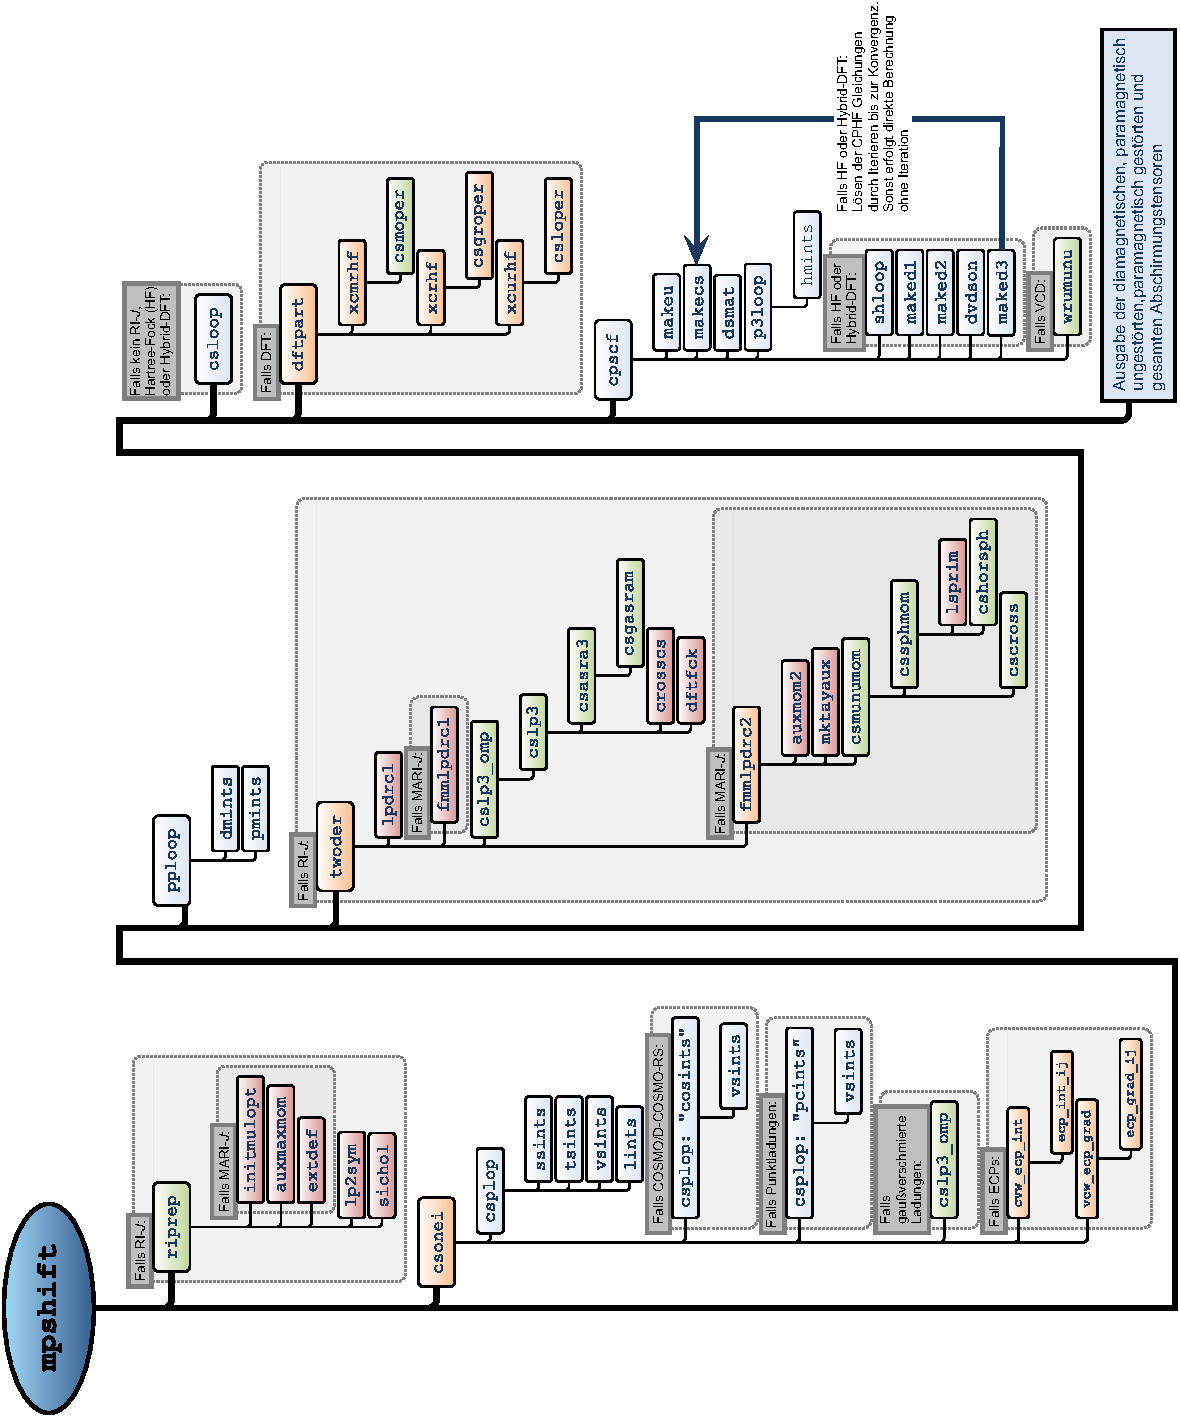
\includegraphics[width=1.1\textwidth]{mpshift_all_seitlich}
	}
	\captionsetup{figurewithin = chapter}
	\captionsetup{font=small, labelfont=bf}\caption[Neue schematische Programmstruktur des Moduls \texttt{mpshift}]{Schematische Programmstruktur des Moduls \texttt{mpshift} mit den wichtigsten Änderungen und Erweiterungen die im Rahmen der vorliegenden Arbeit durchgeführt wurden. Alte Routinen sind in blau, neue Routinen in grün, modifizierte Routinen in orange und unverändert aus anderen Modulen übertragene Routinen in rot dargestellt.}
\label{abb:neue_programmstruktur}
\end{figure}
